\chapter{MapReduce}
\rhead{MapReduce}
\begin{refsection}
\chapterauthor{Daniel Monti, Pascal Stump}

\section{MapReduce}
MapReduce ist ein Programmiermodell, mit dessen Hilfe man sehr grosse
Datenmenge verarbeiten kann.  Die M"oglichkeiten reichen bis zu
einigen Petabyte an Daten \cite{wiki:mapReduce}.

MapReduce wurde urspr"unglich von Google eingef"uhrt, um die riesigen
Datenmengen zu verarbeiten, welche bei der Erstellung der Suchindexe
und Page-Rank-Tabellen entstehen.

Das Problem bei grossen Datenmengen ist weniger der Bedarf von grosser
Rechenleistung, als mehr die Lese- und Schreibzeiten.  Somit kann man
bei MapReduce Problemen Zusammenschl"usse aus ganz \enquote{normaler
  Hardware} verwenden.

F"ur die Arbeitsaufteilung gibt es vorgefertigte
MapReduce-Frameworks.  Eines der Bekanntesten ist zum Beispiel hadoop
\cite{apache:hadoop}.  Es sorgt selbsst"andig f"ur die Aufteilung der
Map-Prozesse und bemerkt verlorene Tasks.

Das MapReduce Konzept arbeitet mit zwei separaten Abl"aufe.
Einerseits gibt es einen parallelen Map Teil und andererseits gibt es
einen nicht parallelen Reduce Teil.  In der Abbildung \ref{MapReduce}
ist der Datenfluss dargestellt, welcher im Folgenden beschrieben wird.

\subsection{Map}
Unstrukturierte Daten werden den parallel laufenden Map Prozessen
"ubergeben.  Daraus werden die Schl"ussel-Werte-Paare generiert und
anschliessend zwischengespeichert.

Diese strukturierten Daten-Paare entsprechen noch nicht dem
Resultat. Es wird erst durch den nachgeschalteten Reduce Prozess
berechnet.

\subsection{Reduce}
Aus den strukturierten Daten, welche die Map Prozesse generiert haben,
kann nun das Resultat berechnet werden.  Dieser Reduce Prozess kann
nicht Parallel ablaufen, da immer "uber den gesamten Datenbestand
berechnet wird.  Es k"onnen aber mehrere Reduce Prozesse gestartet
werden, pro gesuchtes Ergebnis einen.

Man kann also aus den gewonnen Schl"ussel-Werte-Paaren verschiedene
Ergebnisse erzeugen.  Dadurch muss man den Map Prozess nicht f"ur
jedes Ergebnis neu durchlaufen.  Ein Beispiel, soll dies
verdeutlichen.

\begin{figure}
  \begin{center}
  \begin{tikzpicture}
    \node[rectangle,fill=blue!20] (data) {Daten};

    \node[circle,fill=green!80] (map1) [right=of data,yshift=1.5cm,xshift=-.5cm] {Map};
    \node[circle,fill=green!80!black] (map2) [right=of data,xshift=-.5cm] {Map};
    \node[circle,fill=green!60!black] (map3) [right=of data,yshift=-1.5cm,xshift=-.5cm] {Map};

    \node[rectangle,fill=blue!20,align=left] (zData) [right=of map2,xshift=-.5cm] {Zwischen-\\ergebnisse};

    \node[ellipse,fill=orange!40] (reduce1) [right=of zData,yshift=1cm,xshift=-.5cm] {Reduce};
    \node[ellipse,fill=orange!60] (reduce2) [right=of zData,yshift=-1cm,xshift=-.5cm] {Reduce};

    \node[ellipse,fill=orange!40] (erg1) [right=of reduce1,xshift=-.5cm] {Ergebnis};
    \node[ellipse,fill=orange!60] (erg2) [right=of reduce2,xshift=-.5cm] {Ergebnis};

    \draw[->,>=stealth',thick] (data)  to [out=45,in=180]  (map1.west) --++ (7:.01cm);
    \draw[->,>=stealth',thick] (data)  to [out=0,in=180]   (map2);
    \draw[->,>=stealth',thick] (data)  to [out=-45,in=180] (map3.west) --++ (-7:.01cm);

    \draw[->,>=stealth',thick] (map1)  to [out=0,in=135]   (zData);
    \draw[->,>=stealth',thick] (map2)  to [out=0,in=180]   (zData);
    \draw[->,>=stealth',thick] (map3)  to [out=0,in=-135]  (zData);

    \draw[->,>=stealth',thick] (zData) to [out=45,in=180]  (reduce1);
    \draw[->,>=stealth',thick] (zData) to [out=-45,in=180] (reduce2);

    \draw[->,>=stealth',thick] (reduce1) to [out=0,in=180] (erg1);
    \draw[->,>=stealth',thick] (reduce2) to [out=0,in=180] (erg2);
  \end{tikzpicture}
  \end{center}

  \caption{Datenfluss bei MapReduce}
  \label{MapReduce}
\end{figure}


\subsection{Beispiel}
\begin{beispiel}
  Man besitzt Unmengen an Wetterdaten von den letzten Hundert Jahren.
  Man hat nun das Problem, dass man f"ur jedes Jahr die maximalen und
  minimalen Jahresh"ochstwerte ben"otigt. (Beispiel angelehnt an
  \cite{uniLeipzig:mapReduce})

  \begin{enumerate}
    \item Die Daten werden den verschiedenen Map Prozessen
      "ubergeben.  Die Unterteilung k"onnte zum Beispiel so aussehen,
      dass jeder Monat in einer anderen Datei abgespeichert wurde.

      Die Daten k"onnten zum Beispiel ununterbrochene Zahlenfolgen
      sein:
      \begin{center}
        ...201301011300-0072...
      \end{center}
      (\dots{} 01.01.2013 13:00\,Uhr \SI{-7.2}{\degreeCelsius} \dots{})
    \item Jeder Map Prozess arbeitet eine Datei ab (Daten von einem
      Monat).  Daraus generiert jeder Map Prozess die
      Schl"ussel-Werte-Paare.
      \begin{center}
      \begin{tabular}{lr}
        (2013, &-7.2)\\
        (2013, &22)\\
        (2013, &-11)\\
        (2012, &5)
      \end{tabular}
      \end{center}

    \item Diese Schl"ussel-Werte-Paare werden nun
      Zwischengespeichert.

    \item Aus diesen strukturierten Daten kann man mit dem Reduce
      Prozess das gew"unschte Ergebnis berechnen.

      In unserem Fall werden zwei Reduce Prozesse gestartet.  Der eine
      findet zu jedem Schl"ussel die h"ochste, \dots{}
      \begin{center}
      \begin{tabular}{lr}
        (2013, &22)\\
        (2012, &5)
      \end{tabular}
      \end{center}
      \dots{} der andere die tiefste Temperatur.
      \begin{center}
      \begin{tabular}{lr}
        (2013, &-11)\\
        (2012, &5)
      \end{tabular}
      \end{center}
    \item Die Ergebnisse werden ausgegeben.
  \end{enumerate}

\end{beispiel}


\subsection{Shuffle}
Je nach der Implementation des MapReduce Konzepts, gibt es zwischen
dem Map Teil und dem Reduce Teil noch einen Shuffle Prozess.  Dieser
sorgt daf"ur, dass alle gleichen Schl"ussel zusammengefasst werden.

Im Beispiel w"urden nun alle 2013 Schl"ussel zusammengefasst:
\begin{center}
  \begin{tabular}{lrrr}
   (2013, &-7.2, &22, & -11)
  \end{tabular}
\end{center}

Dabei k"onnen beide Reduce Prozesse von der Arbeit des Shuffle
Prozesses profitieren. Da das Zusammensuchen der \enquote{Jahre}
(Schl"ussel) nicht mehr bei jedem Reduce Prozess unabh"angig gemacht
werden muss, sondern nur einmal f"ur alle Reduce Prozesse.







\section{Eigenwertberechnung}
MapReduce eignet sich nicht direkt f"ur die Programmierung numerischer
Algorithmen, da es f"ur die Verarbeitung unstrukturierter Daten
ausgelegt ist, die sich mit Schl"ussel-Wert-Paaren beschreiben lassen.
Die Idee von MapReduce, eine Aufgabe in abwechselende, parallele und
nicht parallele Teilschritte zu zerlegen, l"asst sich durchaus auch in
numerischen Problem anwenden.  Wir zeigen in diesem Kapitel, wie die
Berechnung des PageRank, der nat"urlich ebenfalls mit der Google
Suchmaschine in Zusammenhang steht, mit diesem Konzept parallelisiert
werden kann.

\subsection{Google Matrix und Page Rank}
Die Google Matrix wird verwendet, um die Beliebtheit der verschiedenen
Internetseiten in die Suchabfrage einzubeziehen.  Dieser so genannte
Page Rank ist der Eigenvektor zum gr"ossten Eigenwert der Google
Matrix.  Der gr"osste Eigenwert ist dabei immer 1.  Zudem ist die
Spaltensumme in der Google Matrix 1.

Ein Beispiel soll die Funktionsweise zeigen \cite{mueller:linAlg}
\begin{beispiel}
  In unserem Internet gibt es acht verschiedene Internetseiten (siehe
  Abbildung \ref{bspInternet}):
  \begin{figure}
  \begin{center}
  \begin{tikzpicture}
    [page/.style={circle,draw,semithick},
     connection/.style={->,>=stealth',semithick}]
    \node[page] (nr1) {1};
    \node[page] (nr2) [below=of nr1] {2};

    \node[page] (nr3) [right=of nr1] {3};
    \node[page] (nr4) [below=of nr3] {4};

    \node[page] (nr5) [right=of nr3] {5};
    \node[page] (nr6) [below=of nr5] {6};

    \node[page] (nr7) [right=of nr5] {7};
    \node[page] (nr8) [below=of nr7] {8};


    \draw[connection] (nr1) to (nr2);
    \draw[connection] (nr1) to (nr3);

    \draw[connection,bend left=20] (nr2) to (nr4);

    \draw[connection] (nr3) to (nr2);
    \draw[connection] (nr3) to (nr5);

    \draw[connection,bend left=20] (nr4) to (nr2);
    \draw[connection] (nr4) to (nr5);
    \draw[connection] (nr4) to (nr6);

    \draw[connection] (nr5) to (nr6);
    \draw[connection,bend left=20] (nr5) to (nr7);
    \draw[connection] (nr5) to (nr8);

    \draw[connection,bend left=20] (nr6) to (nr8);

    \draw[connection,bend right=35] (nr7) to (nr1);
    \draw[connection,bend left=20] (nr7) to (nr5);
    \draw[connection,bend left=20] (nr7) to (nr8);

    \draw[connection,bend left=20] (nr8) to (nr6);
    \draw[connection,bend left=20] (nr8) to (nr7);
  \end{tikzpicture}
  \end{center}
  \caption{Beispiel-Internet}
	\label{bspInternet}
  \end{figure}
  
  Daraus l"asst sich eine Matrix $H$ erstellen, welche die
  Wahrscheinlichkeit beschreibt, von einer Internetseite zu einer
  Anderen zu kommen (die so genannte Google Matrix).

\[
    H =
    \begin{pmatrix}
      0 & 0 & 0 & 0 & 0 & 0 & \frac{1}{3} & 0\\
      \frac{1}{2} & 0 & \frac{1}{2} & \frac{1}{3} & 0 & 0 & 0 & 0\\
      \frac{1}{2} & 0 & 0 & 0 & 0 & 0 & 0 & 0\\
      0 & 1 & 0 & 0 & 0 & 0 & 0 & 0\\
      0 & 0 & \frac{1}{2} & \frac{1}{3} & 0 & 0 &
        \frac{1}{3} & 0\\
      0 & 0 & 0 & \frac{1}{3} & \frac{1}{3} & 0 & 0 & \frac{1}{2}\\
      0 & 0 & 0 & 0 & \frac{1}{3} & 0 & 0 & \frac{1}{2}\\
      0 & 0 & 0 & 0 & \frac{1}{3} & 1 & \frac{1}{3} & 0
    \end{pmatrix}
\]

  Von der ersten Internetseite f"uhren Links zur zweiten und dritten
  Internetseite.  Beide Links besitzen die gleiche Wahrscheinlichkeit.
  Somit ist die Wahrscheinlichkeit von der ersten Internetseite zur
  zweiten oder dritten zu kommen je \SI{50}{\percent}.  Zu sehen in
  der Google Matrix in der ersten Spalte und der zweiten/dritten Zeile
  mit dem $\frac{1}{2}$.  Was der ersten Internetseite und den beiden
  Links zur zweiten/dritten Internetseite entspricht.

  Mit der Potenzmethode $u_{k+1} = \frac{Hu_k}{|Hu_k|}$ kann man nun
  die Matrix l"osen und erh"alt den gr"ossten Eigenvektor $u$,
  welcher dem Page Rank entspricht.
\end{beispiel}

\subsection{Potenzmethode}
Als Berechnungsgrundlage benutzen wir die Potenzmethode:
\[
\begin{bmatrix}
u_1 \\
u_2 \\
u_3 \\
u_4 \\
u_5 \\
u_6 \\
u_7 \\
u_8 \\
\end{bmatrix}
=
\begin{bmatrix}
\frac{2}{4} & \frac{1}{4} & 0 & 0 & 0 & 0 & 0 & 0 \\
\frac{2}{4} & \frac{1}{4} & \frac{1}{3} & 0 & 0 & 0 & 0 & 0 \\
0 & \frac{1}{2} & \frac{1}{3} & \frac{1}{5} & 0 & 0 & 0 & 0 \\
0 & 0 & \frac{1}{3} & \frac{3}{5} & \frac{1}{3} & 0 & 0 & 0 \\
0 & 0 & 0 & \frac{1}{5} & \frac{1}{3} & \frac{1}{4} & 0 & 0 \\
0 & 0 & 0 & 0 & \frac{1}{3} & \frac{1}{2} & \frac{2}{6} & 0 \\
0 & 0 & 0 & 0 & 0 & \frac{1}{4} & \frac{3}{6} & \frac{3}{5}\\
0 & 0 & 0 & 0 & 0 & 0 & \frac{1}{6} & \frac{2}{5} \\
\end{bmatrix}
\cdot
\begin{bmatrix}
u_1 \\
u_2 \\
u_3 \\
u_4 \\
u_5 \\
u_6 \\
u_7 \\
u_8 \\
\end{bmatrix}
\]




\[
\textsl{Eigenvektor}(u)=\dfrac{\textsl{Eigenvektor} \cdot \textsl{Matrix}}{\text{norm}(\textsl{Eigenvektor} \cdot \textsl{Matrix})}
\]
\[
\textsl{Eigenwert}\footnote{Betragsm"assig gr"osster Eigenwert} = \textsl{Eigenvektor}^T \cdot \textsl{Matrix} \cdot \textsl{Eigenvektor}
\]

Die Potenzmethode wurde in einem vorherigen Kapitel behandelt. Darum
wird hier nicht n"aher darauf eingegangen.



\subsection{Grundidee}
Bei der Berechnung grosser Matrizen ist zu beachten, dass der
Berechnungsaufwand mit der Gr"osse exponentiell ansteigt und
erhebliche Teile der Berechnungszeit f"ur die Iterationen verwendet
wird.

Die Grundidee ist, eine Bandmatrix diagonal aufzuteilen und den
Potenzalgorithmus auf die Teilmatrizen anzuwenden. Dadurch werden die
Eigenvektoren der Teilmatrizen bestimmt, welche anschliessend in den
gesamten Eigenvektor eingesetzt werden, wie auf Abbildung \ref{1}
ersichtlich ist. Dadurch wird erwartet, dass die Berechnung "uber die
gesamte Matrix mit diesem angepassten Eigenvektor viel weniger
Iterationsschritte ben"otigt als die originale Berechnung ohne
Aufteilung.


\begin{figure}
\begin{center}
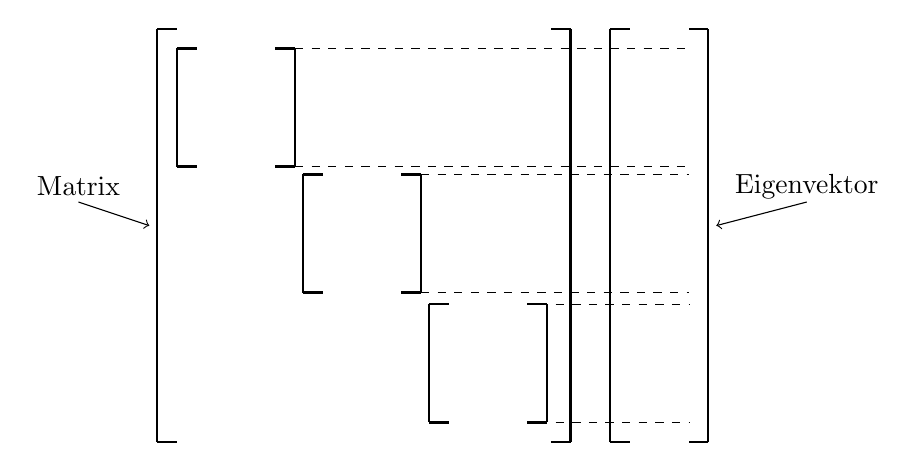
\begin{tikzpicture}[scale = 0.5]
\draw[thick] (0,10) -- (0,-0.5);
\draw[thick] (0,10) -- (0.5,10);
\draw[thick] (0,-0.5) -- (0.5,-0.5);
\draw[thick] (10.5,10) -- (10.5,-0.5);
\draw[thick] (10.5,10) -- (10,10);
\draw[thick] (10,-0.5) -- (10.5,-0.5);
\draw[thick] (0.5,9.5) -- (0.5,6.5);
\draw[thick] (0.5,9.5) -- (1,9.5);
\draw[thick] (0.5,6.5) -- (1,6.5);
\draw[thick] (3.5,9.5) -- (3,9.5);
\draw[thick] (3.5,6.5) -- (3,6.5);
\draw[thick] (3.5,9.5) -- (3.5,6.5);
\draw[thick] (3.7,6.3) -- (3.7,3.3);
\draw[thick] (6.7,6.3) -- (6.7,3.3);
\draw[thick] (3.7,6.3) -- (4.2,6.3);
\draw[thick] (3.7,3.3) -- (4.2,3.3);
\draw[thick] (6.7,3.3) -- (6.2,3.3);
\draw[thick] (6.7,6.3) -- (6.2,6.3);
\draw[thick] (6.9,3) -- (6.9,0);
\draw[thick] (6.9,3) -- (7.4,3);
\draw[thick] (6.9,0) -- (7.4,0);
\draw[thick] (9.9,3) -- (9.9,0);
\draw[thick] (9.9,3) -- (9.4,3);
\draw[thick] (9.9,0) -- (9.4,0);

\draw[thick] (11.5,-0.5) -- (11.5,10);
\draw[thick] (11.5,-0.5) -- (12,-0.5);
\draw[thick] (11.5,10) -- (12,10);
\draw[thick] (14,-0.5) -- (14,10);
\draw[thick] (14,-0.5) -- (13.5,-0.5);
\draw[thick] (14,10) -- (13.5,10);

\draw[dashed] (3.5,9.5) -- (13.5,9.5);
\draw[dashed] (3.5,6.5) -- (13.5,6.5);
\draw[dashed] (6.7,6.3) -- (13.5,6.3);
\draw[dashed] (6.7,3.3) -- (13.5,3.3);
\draw[dashed] (9.7,3) -- (13.5,3);
\draw[dashed] (9.7,0) -- (13.5,0);

\draw (-2,6) node {Matrix};
\draw[<-] (-0.2,5) -- (-2,5.6);
\draw (16.5,6) node {Eigenvektor};
\draw[<-] (14.2,5) -- (16.5,5.6);
\end{tikzpicture}
\end{center}
\caption{Aufteilung der Matrix}
\label{1}
\end{figure}

\subsection{Anf"angliche Versuche}
Bei der ersten Implementation des Codes in Matlab/Octave gingen wird
von der Aufteilung wie in Abbildung \ref{1} aus. Dies konfrontierte
uns aber mit dem Problem, dass in Abbildung \ref{111} ersichtlich
ist. Bei der Diagonalen Aufteilung ergeben sich die roten Dreiecke die
nicht mit gerechnet werden.
 
\begin{figure}
\begin{center}
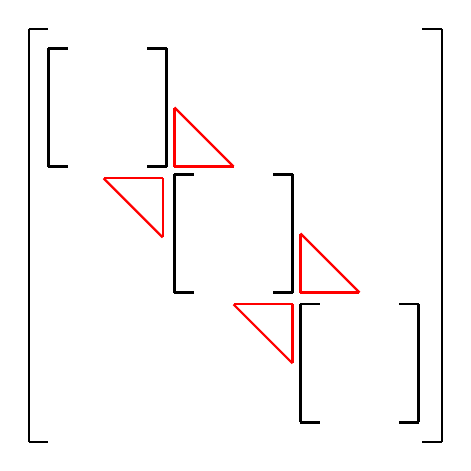
\begin{tikzpicture}[scale = 0.5]
\draw[thick] (0,10) -- (0,-0.5);
\draw[thick] (0,10) -- (0.5,10);
\draw[thick] (0,-0.5) -- (0.5,-0.5);
\draw[thick] (10.5,10) -- (10.5,-0.5);
\draw[thick] (10.5,10) -- (10,10);
\draw[thick] (10,-0.5) -- (10.5,-0.5);
\draw[thick] (0.5,9.5) -- (0.5,6.5);
\draw[thick] (0.5,9.5) -- (1,9.5);
\draw[thick] (0.5,6.5) -- (1,6.5);
\draw[thick] (3.5,9.5) -- (3,9.5);
\draw[thick] (3.5,6.5) -- (3,6.5);
\draw[thick] (3.5,9.5) -- (3.5,6.5);
\draw[thick] (3.7,6.3) -- (3.7,3.3);
\draw[thick] (6.7,6.3) -- (6.7,3.3);
\draw[thick] (3.7,6.3) -- (4.2,6.3);
\draw[thick] (3.7,3.3) -- (4.2,3.3);
\draw[thick] (6.7,3.3) -- (6.2,3.3);
\draw[thick] (6.7,6.3) -- (6.2,6.3);
\draw[thick] (6.9,3) -- (6.9,0);
\draw[thick] (6.9,3) -- (7.4,3);
\draw[thick] (6.9,0) -- (7.4,0);
\draw[thick] (9.9,3) -- (9.9,0);
\draw[thick] (9.9,3) -- (9.4,3);
\draw[thick] (9.9,0) -- (9.4,0);



\draw[thick,red] (3.7,6.5) -- (3.7,8);
\draw[thick,red] (3.7,6.5) -- (5.2,6.5);
\draw[thick,red] (3.7,8) -- (5.2,6.5);

\draw[thick,red] (6.9,3.3) -- (6.9,4.8);
\draw[thick,red] (6.9,3.3) -- (8.4,3.3);
\draw[thick,red] (6.9,4.8) -- (8.4,3.3);

\draw[thick,red] (6.7,3) -- (6.7,1.5);
\draw[thick,red] (6.7,3) -- (5.2,3);
\draw[thick,red] (5.2,3) -- (6.7,1.5);

\draw[thick,red] (3.4,6.2) -- (3.4,4.7);
\draw[thick,red] (3.4,6.2) -- (1.9,6.2);
\draw[thick,red] (1.9,6.2) -- (3.4,4.7);
\end{tikzpicture}
\end{center}
\caption{Dreiecksproblem bei der Aufteilung}
\label{111}
\end{figure}

Dies brachte uns auf den zweiten Versuch, den wir mit der in Abbildung
\ref{11} gezeigten Aufteilung realisierten. Dieser Code f"uhrte aber
dazu, dass unsere Bearbeitung nur gleich schnell oder teilweise sogar
langsamer war als die original Matrix. Das Problem war, dass die
Aufteilung zu aufwendig war und so kein Zeitgewinn erreicht werden
konnte. Da die Matrix jetzt fast zweimal aufgeteilt wird verdoppelt
sich damit nat"urlich die ben"otigte Zeit. Nach mehreren misslungenen
Versuchen mit und ohne dieser Aufteilung musste wir den L"osungsansatz
fallen lassen, da auch noch ein Problem mit der Normierung vorhanden
war.

\begin{figure}
\begin{center}
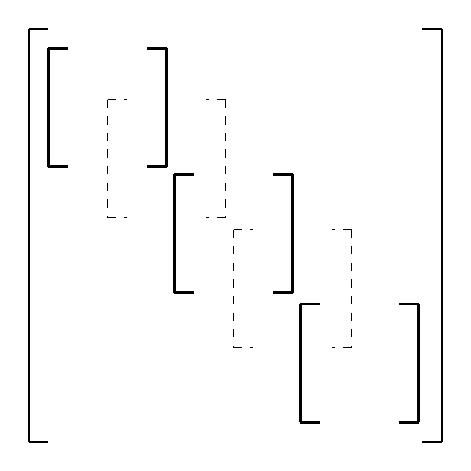
\begin{tikzpicture}[scale = 0.5]
\draw[thick] (0,10) -- (0,-0.5);
\draw[thick] (0,10) -- (0.5,10);
\draw[thick] (0,-0.5) -- (0.5,-0.5);
\draw[thick] (10.5,10) -- (10.5,-0.5);
\draw[thick] (10.5,10) -- (10,10);
\draw[thick] (10,-0.5) -- (10.5,-0.5);
\draw[thick] (0.5,9.5) -- (0.5,6.5);
\draw[thick] (0.5,9.5) -- (1,9.5);
\draw[thick] (0.5,6.5) -- (1,6.5);
\draw[thick] (3.5,9.5) -- (3,9.5);
\draw[thick] (3.5,6.5) -- (3,6.5);
\draw[thick] (3.5,9.5) -- (3.5,6.5);
\draw[thick] (3.7,6.3) -- (3.7,3.3);
\draw[thick] (6.7,6.3) -- (6.7,3.3);
\draw[thick] (3.7,6.3) -- (4.2,6.3);
\draw[thick] (3.7,3.3) -- (4.2,3.3);
\draw[thick] (6.7,3.3) -- (6.2,3.3);
\draw[thick] (6.7,6.3) -- (6.2,6.3);
\draw[thick] (6.9,3) -- (6.9,0);
\draw[thick] (6.9,3) -- (7.4,3);
\draw[thick] (6.9,0) -- (7.4,0);
\draw[thick] (9.9,3) -- (9.9,0);
\draw[thick] (9.9,3) -- (9.4,3);
\draw[thick] (9.9,0) -- (9.4,0);

\draw[dashed] (2,8.2) -- (2,5.2);
\draw[dashed] (2,8.2) -- (2.5,8.2);
\draw[dashed] (2,5.2) -- (2.5,5.2);
\draw[dashed] (5,8.2) -- (5,5.2);
\draw[dashed] (5,5.2) -- (4.5,5.2);
\draw[dashed] (5,8.2) -- (4.5,8.2);

\draw[dashed] (5.2,4.9) -- (5.2,1.9);
\draw[dashed] (5.2,4.9) -- (5.7,4.9);
\draw[dashed] (5.2,1.9) -- (5.7,1.9);
\draw[dashed] (8.2,4.9) -- (8.2,1.9);
\draw[dashed] (8.2,4.9) -- (7.7,4.9);
\draw[dashed] (8.2,1.9) -- (7.7,1.9);
\end{tikzpicture}
\end{center}
\caption{Erster Probleml"osungsversuch}
\label{11}
\end{figure}

\subsection[Algorithmus]{Funktionierender Algorithmus}
Wir wurden mit dem Problem konfrontiert, dass das Potenzverfahren
versucht unbedeutende Vektorkomponenten klein zu machen. Durch die
Renormierung in den Teilmatrizen werden die Teilvektoren auf eine
bestimmte Gr"osse gebracht. Wobei unbedeutende Teilvektoren wieder
gross gemacht werden. Dadurch bewirkt man also genau das Gegenteil
dessen, was der Potenzalgorithmus anstrebt.  Diesen Umstand liessen
wir in den neuen L"osungsansatz einfliessen. Die Abbildung \ref{12}
zeigt pr"azise die Funktion des neuen Algorithmus auf.

\begin{figure}
\begin{center}
 \begin{tikzpicture}
  \node[rectangle,fill=blue!20,draw=blue!50,ultra
  thick,align=center,rounded corners=3mm] (matrix) {pseudo Google
    Matrix generieren};

  % ganze Matrix
  \node[below=of matrix,xshift=-1cm] (original){};
  \node at (original){n};
  \draw[->,>=stealth',very thick,green!40!black](original) ++(-175:.3cm) 
    arc (-175:120:.3cm) --++ (195:.1cm);
  \node[left=of original,xshift=.5cm,align=left] {Gesamt Matrix\\ mit Normierung};

  % Teilmatrix
  \node[below=of matrix,xshift=1cm] (teil10) {};
  \node at (teil10){10};
  \draw[->,>=stealth',very thick,blue!50!black] (teil10) ++(-175:.3cm)
    arc (-175:120:.3cm) --++ (195:.1cm);
  \node[right=of teil10,xshift=-.5cm,align=left] {Teilmatrizen\\ ohne Normierung};
  \node[right=of teil10,xshift=2.8cm,align=left] {Parallel};

  \node[below=of teil10] (gesamt1) {};
  \node at (gesamt1) {1};
  \draw[->,>=stealth',very thick,brown!40!black] (gesamt1) ++ (-175:.3cm)
    arc (-175:120:.3cm) --++ (195:.1cm);
  \node[right=of gesamt1,xshift=-.5cm,align=left] {Gesamt Matrix\\ mit Normierung};
\node[right=of gesamt1,xshift=2.8cm,align=left] {Seriel};

  \node[below=of gesamt1] (teilN) {};
  \node at (teilN) {n};
  \draw[->,>=stealth',very thick,orange!80!black] (teilN) ++ (-175:.3cm)
    arc (-175:120:.3cm) --++ (195:.1cm);
  \node[right=of teilN,xshift=-.5cm,align=left] {Teilmatrizen\\ ohne Normierung};
   \node[right=of teilN,xshift=2.8cm,align=left] {Parallel};

  \node[below=of teilN] (gesamtN) {};
  \node at (gesamtN) {n};
  \draw[->,>=stealth',very thick,green!40!black] (gesamtN) ++ (-175:.3cm)
    arc (-175:120:.3cm) --++ (195:.1cm);
  \node[right=of gesamtN,xshift=-.5cm,align=left] {Gesamt Matrix\\ mit Normierung};
  \node[right=of gesamtN,xshift=2.8cm,align=left] {Seriel};

  % Verbindungen
  \draw[->,>=stealth',thick,shorten >=.3cm,shorten <=.4cm] (matrix) ++
    (180:1cm) to (original);

  \draw[->,>=stealth',thick,shorten >=.3cm,shorten <=.4cm] (matrix) ++
    (0:1cm) to (teil10);
  \draw[->,>=stealth',thick,shorten >=.3cm,shorten <=.3cm] (teil10) to
    (gesamt1);
  \draw[->,>=stealth',thick,shorten >=.3cm,shorten <=.3cm] (gesamt1) to
    (teilN);
  \draw[->,>=stealth',thick,shorten >=.3cm,shorten <=.3cm] (teilN) to
    (gesamtN);
  \end{tikzpicture}
    \end{center}
\caption{Der Algorithmus}
\label{12}
\end{figure}

Zur Kontrolle wird die Matrix ganz normal mit der Potenzmethode
berechnet bis die Genauigkeit von $10^{-4}$ erreicht wurde.

Die pseudo Google Matrix, eine Bandmatrix mit Spaltensumme 1, wird
diagonal aufgeteilt und die Teilmatrizen werden zehn mal mit der
Potenzmethode ohne Normierung berechnet. Die Ergebnisse werden in den
Eigenvektor der gesamt Matrix eingef"ugt. Danach wird die ganze Matrix
mit diesem Eigenvektor berechnet. Dies geschieht mit Normierung und
f"uhrt dazu, dass die komplette Matrix berechnet wird und somit die
anf"anglich gezeigten roten Dreiecke auch einbezogen werden. Danach
werden die Teilmatrizen nochmal berechnet, solange bis die Genauigkeit
von $10^{-4}$ oder die maximale Iterationsanzahl von 10'000
Durchg"angen erreicht ist. Schlussendlich wir "uber die ganze Matrix
iteriert bis die Genauigkeit erreicht ist. Die letzte Iteration
ben"otigt einen Bruchteil der Iterationsschritte im Vergleich zur
originalen Matrix. In Zahlen ausgedr"uckt bedeutet das, dass die
original Matrix ($10^3\times10^3$) 9305 Schritte und die bearbeitete
27 Schritte ben"otigte. Aus dieser Reduktion der Iterationsschritten
ergibt sich der relativ grosse Berechnungszeitgewinn. Da die
Berechnungen "uber die gesamte Matrix sehr aufw"andig sind.

\subsection[Auswertung]{Auswertung der Berechnungszeiten}
Um eine Auswertung des erarbeiteten Algorithmus zu erreichen wollten
wir denn Code 100 mal mit verschiedenen Teilmatrix-Gr"ossen
durchlaufen lassen. Daraus ergeben sich relativ gute
Durchschnittswerte, welche in den folgenden Plots ersichtlich
sind. Die Plots mit $10^2\times10^2$ und $10^3\times10^3$ gingen 100
mal durch. Bei der Matrix mit $10^4\times10^4$ beschr"ankten wir uns
Aufgrund des enormen Rechenaufwands auf nur 5 Durchg"ange.

\begin{figure}
\begin{center}
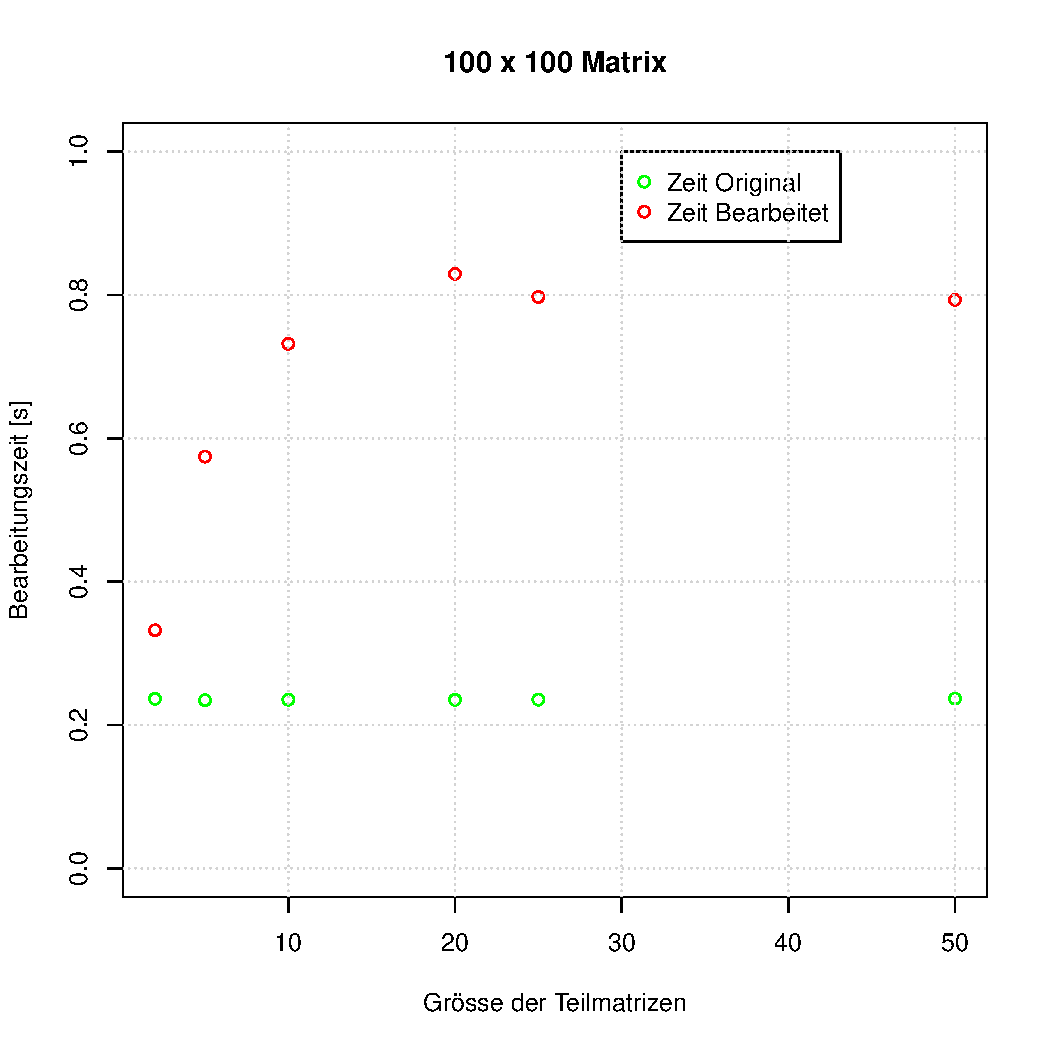
\includegraphics[width=0.7\textwidth]{./mapreduce/PC100.pdf}
\end{center}
\caption{Auswertungs Plot $100\times100$}
\label{q}
\end{figure}

Aus der Abbildung \ref{q} ist ersichtlich, dass die $10^2\times10^2$
Matrix nicht f"ur die Parallelisierung mit unserer Methode geeignet
ist. Dies ist einfach mit der Gr"osse der Matrix zu erkl"aren. Da die
Aufteilung mehr Zeit ben"otigt als die Berechnung "uber die gesamte
Matrix.

\begin{figure}
\begin{center}
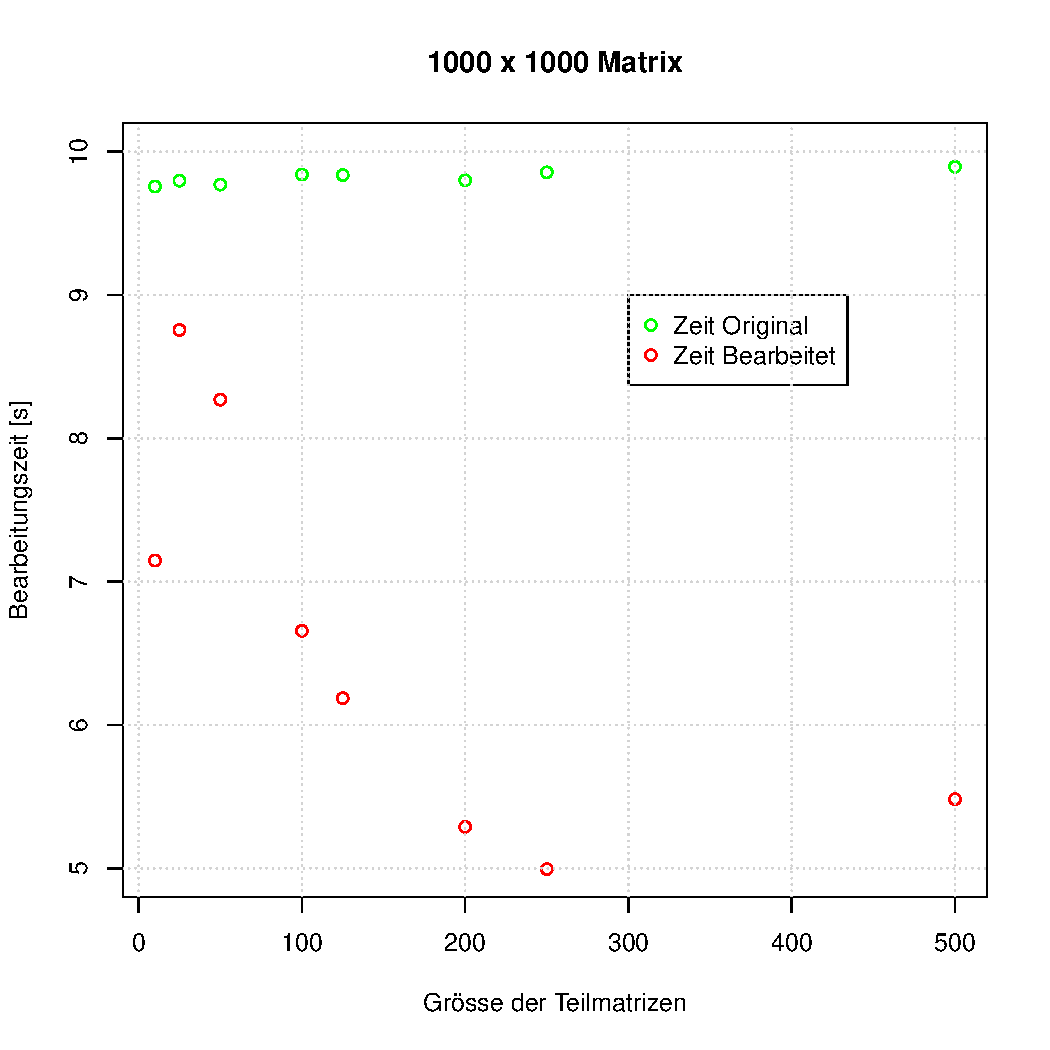
\includegraphics[width=0.7\textwidth]{./mapreduce/PC1000.pdf}
\end{center}
\caption{Auswertungs Plot $1000\times1000$}
\label{qq}
\end{figure}

Bei der $10^3\times10^3$ Matrix sieht das Ergebnis schon besser aus
(Abbildung \ref{qq}). Der Aufteilungsaufwand rechnet sich und ergibt
Geschwindigkeitsfortschritte. Die schnellste Aufteilung ergibt sich
bei einer Teilmatrizen-Gr"osse von $250\times250$. Bei dieser Gr"osse
k"onnen wir die ben"otigte Berechnungszeit halbieren (50.68\% der
Originalzeit). Die verl"angerte Berechnungszeit bei kleineren
Teilmatrizen-Gr"ossen sehen wir in Verbindung mit dem erh"ohten
Aufteilungsaufwand.

\begin{figure}
\begin{center}
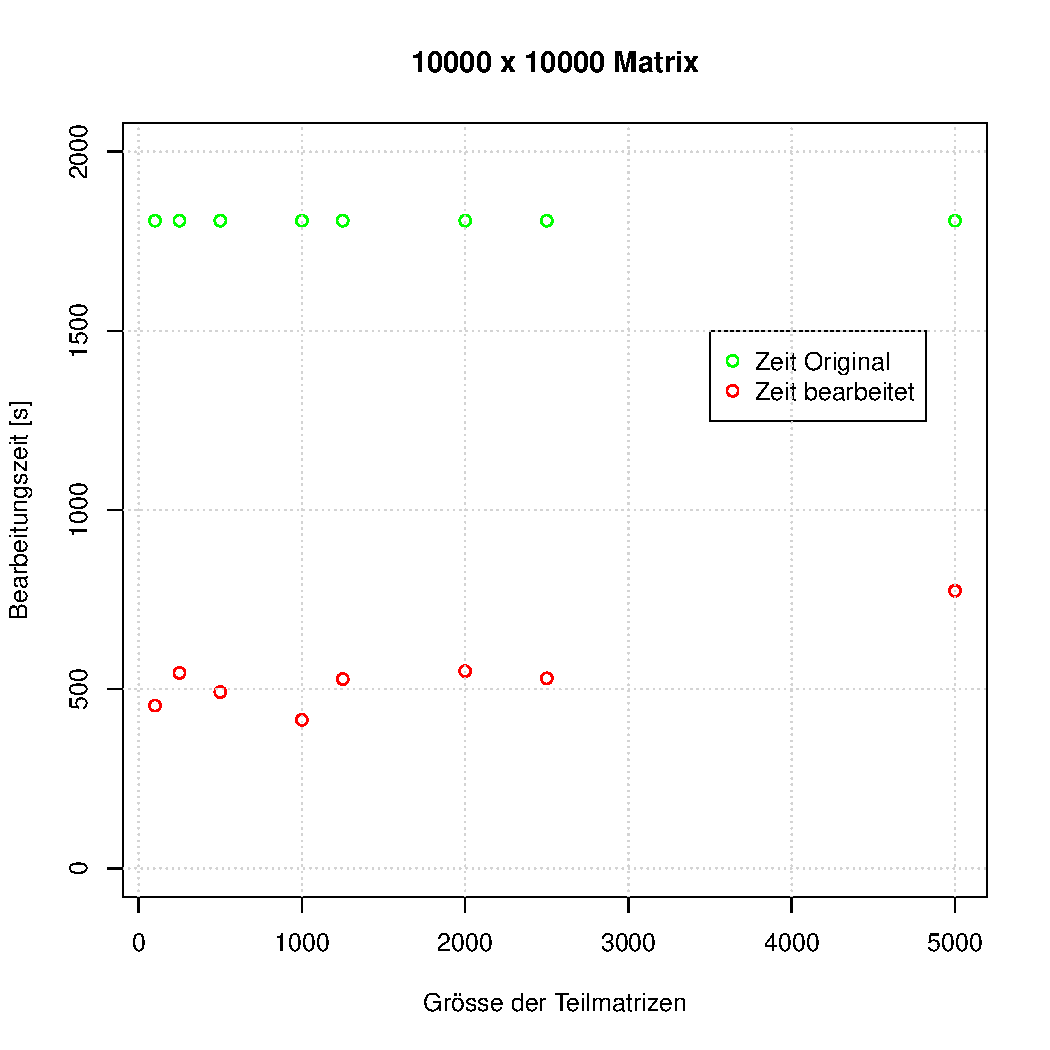
\includegraphics[width=0.7\textwidth]{./mapreduce/PC10000.pdf}
\end{center}
\caption{Auswertungs Plot $10000\times10000$}
\label{qqq}
\end{figure}

Der Plot in der Abbildung \ref{qqq} der $10^4\times10^4$ Matrix zeigt
auch ein erfolgreiches Verfahren. Die Aufteilung mit den
$1000\times1000$ Teilmatrizen l"asst die Berechnungszeit auf
$\frac{1}{4}$ schrumpfen.  An der Berechnungszeit der Originalmatirx
(ca. 27 min) l"asst sich der Rechnungsaufwand erahnen. Trotzdem w"are
unser Algorithmus in realen Verh"altnissen nicht einsetzbar, da er zu
langsam ist. Aber es handelt sich bei unserem Code auch nur um eine
Umsetzung in Matlab/Octave. Eine Implementation in C++ w"are ein
n"achstes Ziel gewesen.

\subsection[Iterationsschritte]{Einfluss der Iterationsschritte}
Im Code werden die Iterationen mit einer maximal Anzahl von
Durchg"angen (10'000) oder bei erreichen der Genauigkeit von $10^{-4}$
abgebrochen. Bei der Anpassung dieser maximalen Iterationsgrenze ist
auch mit einer Beeinflussung der Geschwindigkeit zu rechnen. In den
folgenden Plots wurde genau dies "uberpr"uft.

\begin{figure}
\begin{center}
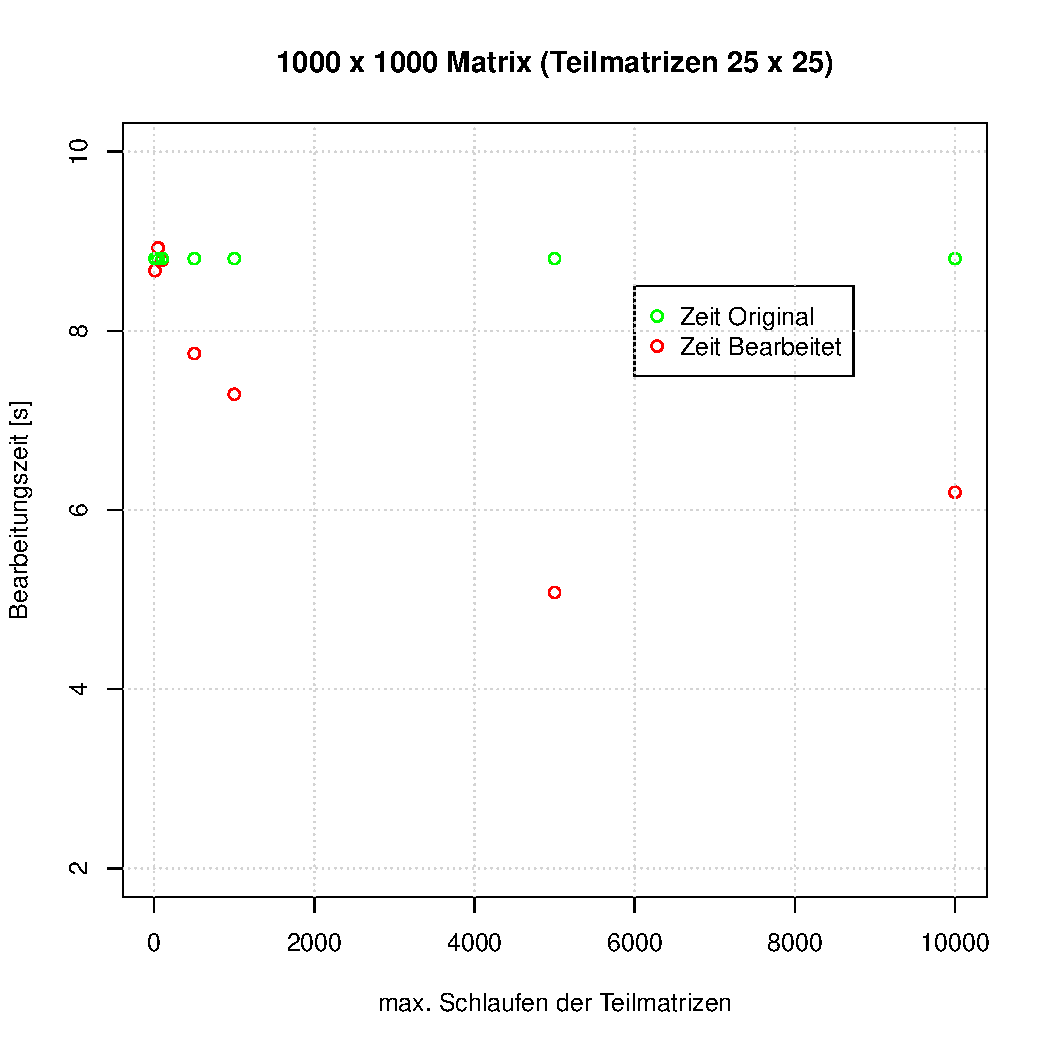
\includegraphics[width=0.7\textwidth]{./mapreduce/PC1000spec25.pdf}
\end{center}
\caption{Reduktion der maximalen Iterationsschritte ($25\times25$ Teilmatrizen)}
\label{w}
\end{figure}

Wie man beim Plot \ref{w} sehr gut sehen kann, bewirkt die
Herabsetzung der Grenze auf 5'000 einen Geschwindigkeitsgewinn. Eine
weiter Herabsetzung f"uhrt jedoch dazu, dass mehr zeitintensive
Iterationen "uber die gesamte Matrix am Schluss berechnet werden
m"ussen, anstatt nur "uber die kleinen Teilmatrizen. Deshalb ist davon
abzuraten die Grenze noch mehr zu verkleinern.

\begin{figure}
\begin{center}
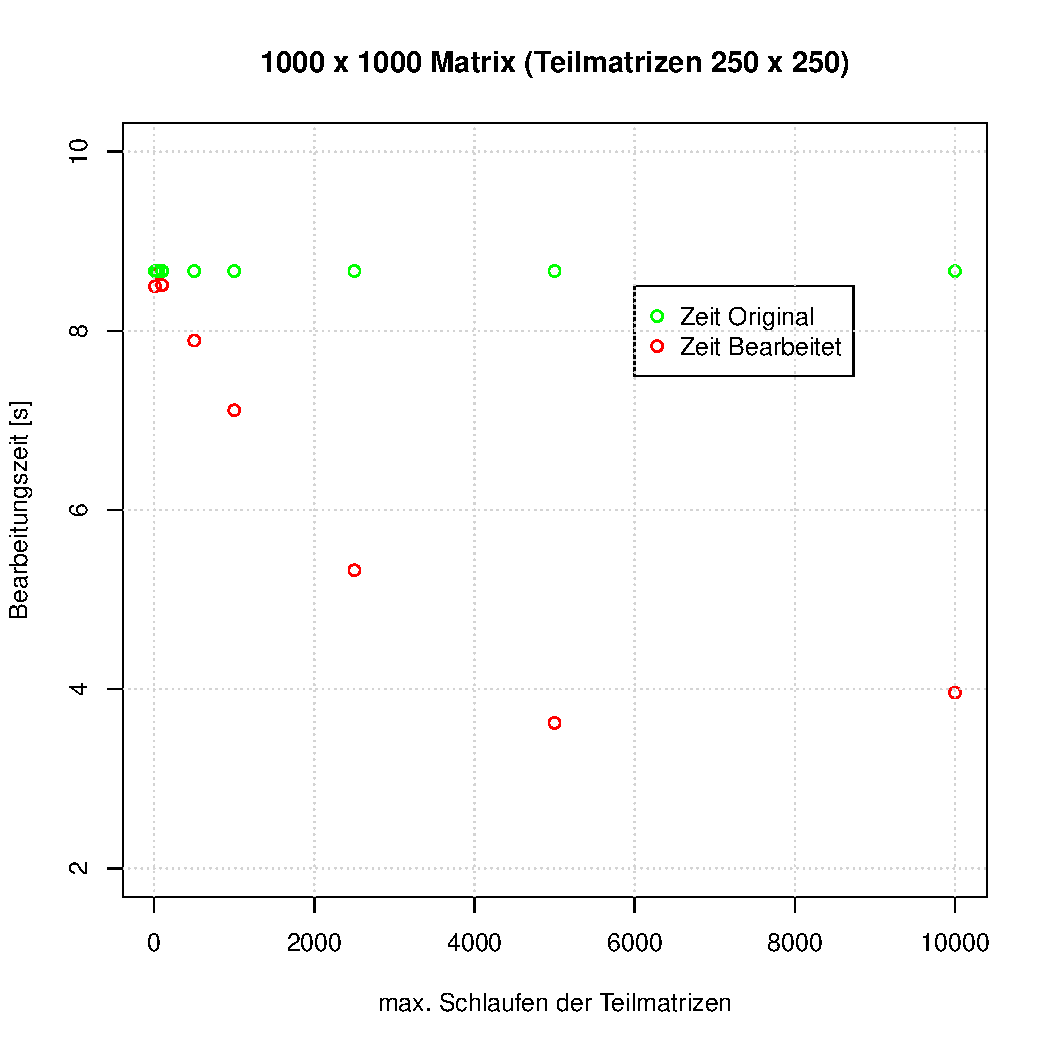
\includegraphics[width=0.7\textwidth]{./mapreduce/PC1000spec250.pdf}
\end{center}
\caption{Reduktion der maximalen Iterationsschritte ($250\times250$ Teilmatrizen)}
\label{ww}
\end{figure}

Ein sehr "ahnliches Bild ist bei den $250\times250$ Teilmatrizen zu
erkennen (Abbildung \ref{ww}). Auch hier f"uhrt eine Halbierung der
Iterationen zu einem Geschwindigkeitsgewinn. Jedoch tritt das selbe
Symptom wie vorher auf. Dennoch kann diese Art der Anpassung je nach
Situation einen Zeitgewinn mit sich f"uhren.

\subsection{Fazit}
Als Fazit aus unseren Versuchen mit dem Eigenwertproblem und MapReduce
k"onnen wir sagen, dass wir es geschafft haben einen funktionierenden
Algorithmus zu implementieren. Dieser ist jedoch in einem fr"uhen
Stadium und noch ausbauf"ahig. Ein n"achster Schritt w"are die
Implementation in einer Hochsprache. So w"are auch eine bessere
Parallelisierung m"oglich gewesen.

Dennoch zeigt der Algorithmus sehr gut, was alles m"oglich ist und wie
die Funktionsweise von MapReduce ist.

\printbibliography[heading=subbibliography]
\end{refsection}

